% Nêu nội dung thực hiện và phương pháp dự kiến để đánh giá hệ thống, ví dụ, nếu KLTN có chạy demo thì hệ thống demo sẽ như thế nào

% Định nghĩa 3-4 nội dung chính

\subsection{Nội dung 1: Triển khai hạ tầng MLOps}

\begin{itemize}
    \item \textbf{Mục tiêu:}
    Giai đoạn này nhằm xây dựng nền tảng hạ tầng cloud-native làm cơ sở cho toàn bộ hệ thống MLOps, đảm bảo các đặc tính về khả năng mở rộng, tính sẵn sàng cao, tự động hoá và khả năng tái lập môi trường. Cụ thể, các mục tiêu chính bao gồm: 

        \begin{itemize}
        \item Thiết lập môi trường container orchestration trên nền tảng Kubernetes để quản lý tài nguyên tính toán cho các pipeline huấn luyện và suy luận.
        \item Xây dựng hạ tầng theo mô hình Infrastructure as Code (IaC) nhằm đảm bảo tính nhất quán, tự động hoá và khả năng tái tạo.
        \item Triển khai hệ thống lưu trữ trung tâm cho dữ liệu, artifact, model và logs.
        \item Thiết lập container registry để quản lý và phân phối các image phục vụ pipeline và model serving.
        \item Chuẩn bị các thành phần nền tảng phục vụ cho các giai đoạn tiếp theo như experiment tracking, pipeline orchestration, CI/CD và model serving.
    \end{itemize}

    \item \textbf{Phương pháp thực hiện:}
        \begin{itemize}
            \item Triển khai cụm Kubernetes bằng cách sử dụng dịch vụ EKS của AWS làm nền tảng điều phối container để quản lý các dịch vụ và pipeline.
            \item Áp dụng Terraform để định nghĩa và triển khai hạ tầng dưới dạng mã (IaC).
            \item Triển khai object storage để lưu trữ.
            \item Thiết lập container registry.
            \item Triển khai MLflow Tracking Server.
            \item Thiết lập Git repository làm nguồn quản lý mã nguồn.
            \item Cấu hình CI pipeline bằng cách sử dụng GitHub Actions.
            \item Triển khai ArgoCD theo mô hình GitOps.
        \end{itemize}
\end{itemize}

\subsubsection{Nội dung 2: Xây dựng CI/CD pipeline}

\begin{itemize}
    \item \textbf{Mục tiêu:}
    Giai đoạn này nhằm xây dựng quy trình tích hợp liên tục (CI) và triển khai liên tục (CD) cho hệ thống MLOps, đảm bảo tự động hoá từ khâu thay đổi mã nguồn, huấn luyện lại mô hình, đến triển khai mô hình vào môi trường phục vụ. Mục tiêu chính bao gồm: 
        \begin{itemize}
            \item Tự động hoá quá trình build, kiểm thử và đóng gói các thành phần pipeline.
            \item Triển khai mô hình theo cơ chế GitOps để tăng khả năng kiểm soát và truy vết
            \item Giảm thiểu sự can thiệp thủ công trong quá trình cập nhật hệ thống.
        \end{itemize}
    
    \item \textbf{Phương pháp thực hiện:}
        \begin{itemize}
            \item Xây dựng quy trình CI/CD dựa trên kiến trúc pipeline tự động kết hợp với mô hình GitOps.
            \item Quản lý toàn bộ mã nguồn pipeline, cấu hình hạ tầng và thành phần triển khai trên Github.
            \item Tự động kích hoạt quy trình CI khi có thay đổi mã nguồn, bao gồm kiểm thử, build Docker image và đóng gói các thành phần phục vụ huấn luyện và triển khai mô hình.
            \item Đẩy các Docker image sau khi build thành công lên container registry để phục vụ các môi trường triển khai.
            \item Triển khai CD theo mô hình GitOps, trong đó trạng thái mong muốn của hệ thống được định nghĩa bằng các tập tin K8s manifest hoặc Helm chart trong kho lưu trữ.
            \item Tự động đồng bộ cấu hình từ repository vào cụm Kubernetes để triển khai hoặc cập nhật pipeline và dịch vụ model serving.
\end{itemize}

\end{itemize}

\subsection{Nội dung 3: Thu nhập, xử lý dữ liệu và phát triển mô hình}

\begin{itemize}
    \item \textbf{Mục tiêu:} 
     Giai đoạn này nhằm xây dựng quy trình xử lý dữ liệu và phát triển mô hình học máy theo hướng có thể tái lập, theo dõi và tự động hoá. Cụ thể, mục tiêu bao gồm: 
        \begin{itemize}
             \item Thiết lập quy trình thu thập và quản lý dữ liệu đầu vào.
             \item Chuẩn hoá các bước tiền xử lý và trích xuất đặc trưng.
             \item Xây dựng môi trường thử nghiệm để huấn luyện và tinh chỉnh mô hình; 
             \item Theo dõi toàn bộ quá trình thử nghiệm nhằm đảm bảo khả năng tái lập kết quả.
             \item Đồng thời tạo ra các mô hình đã được đánh giá và sẵn sàng đưa vào pipeline tự động trong các giai đoạn tiếp theo.
        \end{itemize}
    
    \item \textbf{Phương pháp thực hiện:}
        \begin{itemize}
            \item Thu thập dữ liệu từ các nguồn đầu vào và lưu trữ trong hệ thống object storage.
            \item Quản lý phiên bản dữ liệu nhằm đảm bảo tính truy vết và khả năng tái lập.
            \item Thực hiện tiền xử lý dữ liệu gồm làm sạch, chuẩn hoá và trích xuất đặc trưng.
            \item Lưu trữ đặc trưng trong feature store để sử dụng thống nhất cho huấn luyện và suy luận.
            \item Phát triển và huấn luyện mô hình trong môi trường notebook.
            \item Theo dõi các thí nghiệm thông qua hệ thống experiment tracking, ghi nhận tham số, chỉ số đánh giá và artifact.
            \item Đánh giá mô hình theo các tiêu chí định lượng và đóng gói các mô hình đạt yêu cầu để chuyển sang giai đoạn xây dựng pipeline, đăng ký và triển khai.
        \end{itemize}

\end{itemize}

\subsubsection{Nội dung 4: Giám sát và ghi nhận kết quả}

\begin{itemize}
    \item \textbf{Mục tiêu:}
    Giai đoạn này nhằm thiết lập cơ chế giám sát toàn diện cho hệ thống MLOps và đánh giá hiệu quả của mô hình trong môi trường thực tế. Mục tiêu chính bao gồm: theo dõi trạng thái hoạt động của hệ thống và dịch vụ mô hình; \
        \begin{itemize}
            \item Giám sát các chỉ số hiệu năng 
            \item Phát hiện sự thay đổi phân phối dữ liệu đầu vào hoặc sự suy giảm chất lượng dự đoán của mô hình.
            \item Tổng hợp kết quả triển khai để đánh giá mức độ đáp ứng các yêu cầu của hệ thống MLOps đề ra ban đầu.
        \end{itemize}
    
    \item \textbf{Phương pháp thực hiện:}
        \begin{itemize}
            \item Triển khai hệ thống giám sát theo hai lớp: giám sát hạ tầng và giám sát mô hình.
            \item Thu thập và trực quan hoá các chỉ số hạ tầng như CPU, bộ nhớ, độ trễ và số lượng yêu cầu của dịch vụ suy luận.
            \item Giám sát dữ liệu đầu vào và đầu ra của mô hình nhằm phát hiện các hiện tượng như data drift.
            \item Kích hoạt lại pipeline huấn luyện khi phát hiện dấu hiệu suy giảm chất lượng mô hình.
        \end{itemize}
\end{itemize}

\begin{figure}[!h]
    \centering
    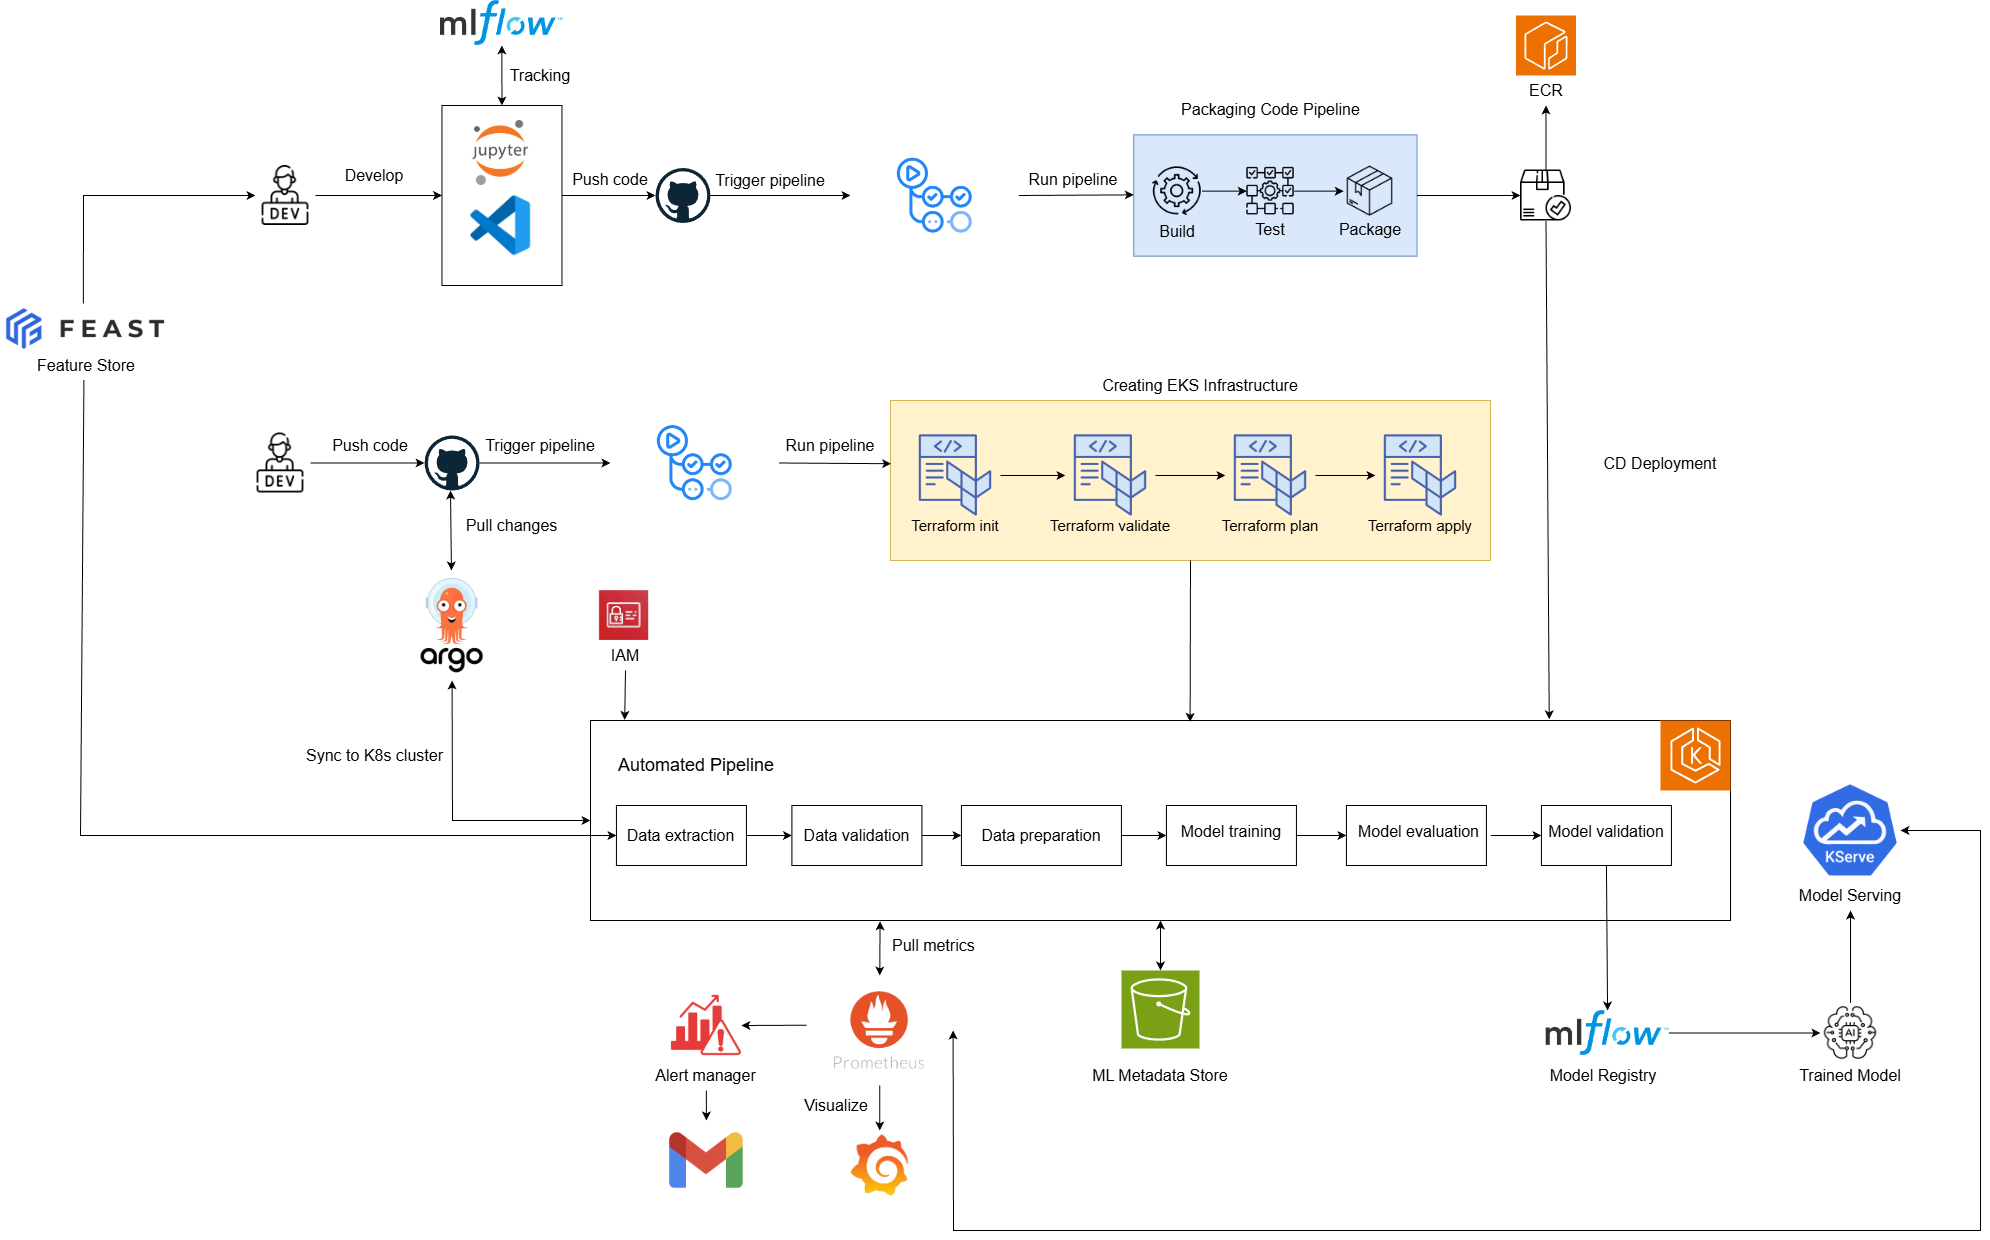
\includegraphics[width=0.95\linewidth]{Figures/KLTN - BaoDHG - BaoTG - MLOps Architecture.drawio.png}
    \caption{Hệ thống triển khai}
    \label{fig:deployed-system}
\end{figure}

\subsubsection{Giới hạn của đề tài}

Mặc dù hệ thống MLOps được xây dựng nhằm đáp ứng các yêu cầu về tự động hóa và quản lý vòng đời mô hình, đề tài vẫn tồn tại một số hạn chế. Do giới hạn về thời gian và nguồn lực, dữ liệu và phạm vi thực nghiệm chưa đủ lớn để phản ánh toàn diện các tình huống thực tế. Tài nguyên tính toán còn hạn chế nên chưa thể thực hiện các thí nghiệm và tối ưu ở quy mô sâu và đa dạng. Ngoài ra, hệ thống mới được kiểm chứng ở mức thử nghiệm, chưa đánh giá đầy đủ trong môi trường vận hành thực tế với quy mô lớn và thời gian dài.